\chapter{Joshua 20}

\begin{figure}
  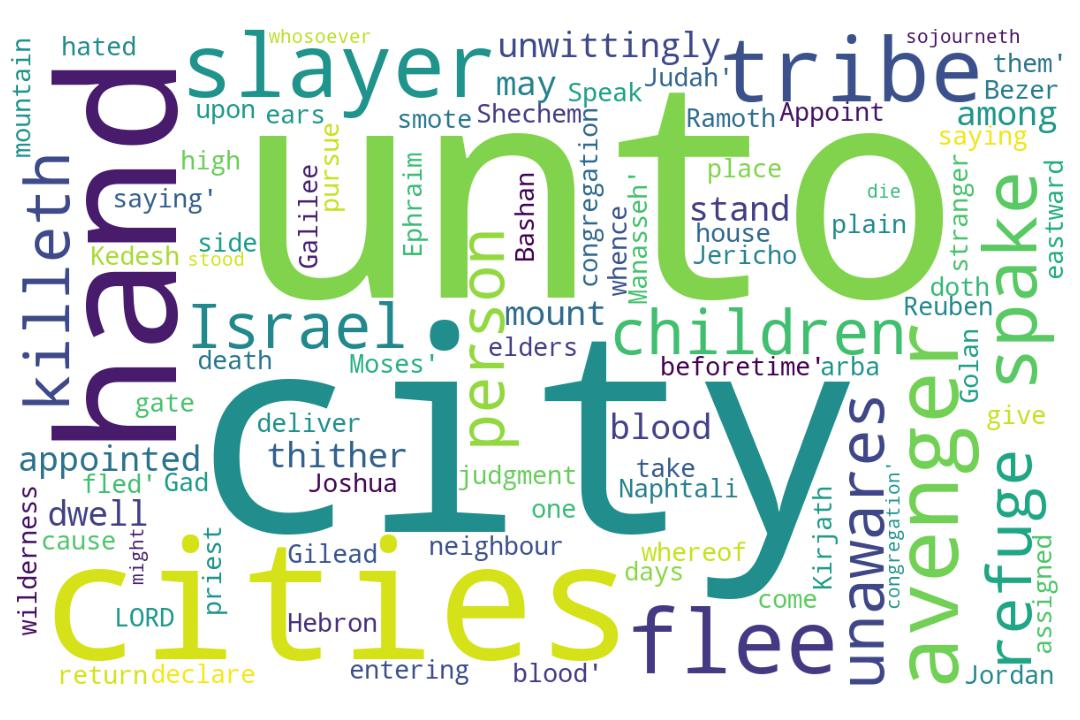
\includegraphics[width=\linewidth]{06OT-Joshua/Joshua20-WordCloud.jpg}
  \caption{Joshua 20 Word Cloud}
  \label{fig:Joshua 20 Word Cloud}
\end{figure}

\marginpar{\scriptsize \centering \fcolorbox{blue}{lime}{\textbf{CITIES OF REFUGE}}\\ (Joshua 20)

\begin{compactenum}[I.][8]

    \item \textbf{Presumptions}  \index[scripture]{Joshua!Jsh 20:03}(Jsh 20:3)
    \item \textbf{Persons} Killed \index[scripture]{Joshua!Jsh 20:03} \index[scripture]{Joshua!Jsh 20:09} (Jsh 20:3, 9)
    \item A \textbf{Place} of Refuge \index[scripture]{Joshua!Jsh 20:04}(Jsh 20:4)
    \item Being \textbf{Pursued}  \index[scripture]{Joshua!Jsh 20:05}(Jsh 20:5)
    \item The \textbf{Life} of the Priest \index[scripture]{Joshua!Jsh 20:06}(Jsh 20:6)
    \item The \textbf{Plain} of Reuben \index[scripture]{Joshua!Jsh 20:08}(Jsh 20:8)
   \item \textbf{Protection}  %\index[scripture]{Joshua!Jsh 20:03}(Jsh 20:3)

\end{compactenum}}





\footnote{\textcolor[rgb]{0.00,0.25,0.00}{\hyperlink{TOC}{Return to end of Table of Contents.}}}\footnote{\href{https://audiobible.com/bible/joshua_20.html}{\textcolor[cmyk]{0.99998,1,0,0}{Joshua 20 Audio}}}\textcolor[cmyk]{0.99998,1,0,0}{The LORD also spake unto Joshua, saying,}
[2] \textcolor[cmyk]{0.99998,1,0,0}{Speak to the children of Israel, saying, Appoint out for you cities of refuge, whereof I spake unto you by the hand of Moses:}
[3] \textcolor[cmyk]{0.99998,1,0,0}{That the slayer that killeth \emph{any} person unawares \emph{and} unwittingly may flee thither: and they shall be your refuge from the avenger of blood.}
[4] \textcolor[cmyk]{0.99998,1,0,0}{And when he that doth flee unto one of those cities shall stand at the entering of the gate of the city, and shall declare his cause in the ears of the elders of that city, they shall take him into the city unto them, and give him a place, that he may dwell among them.}
[5] \textcolor[cmyk]{0.99998,1,0,0}{And if the avenger of blood pursue after him, then they shall not deliver the slayer up into his hand; because he smote his neighbour unwittingly, and hated him not beforetime.}
[6] \textcolor[cmyk]{0.99998,1,0,0}{And he shall dwell in that city, until he stand before the congregation for judgment, \emph{and} until the death of the high priest that shall be in those days: then shall the slayer return, and come unto his own city, and unto his own house, unto the city from whence he fled.}\\
\\
\P \textcolor[cmyk]{0.99998,1,0,0}{And they appointed Kedesh in Galilee in mount Naphtali, and Shechem in mount Ephraim, and Kirjath-arba, which \emph{is} Hebron, in the mountain of Judah.}
[8] \textcolor[cmyk]{0.99998,1,0,0}{And on the other side Jordan by Jericho eastward, they assigned Bezer in the wilderness upon the plain out of the tribe of Reuben, and Ramoth in Gilead out of the tribe of Gad, and Golan in Bashan out of the tribe of Manasseh.}
[9] \textcolor[cmyk]{0.99998,1,0,0}{These were the cities appointed for all the children of Israel, and for the stranger that sojourneth among them, that whosoever killeth \emph{any} person at unawares might flee thither, and not die by the hand of the avenger of blood, until he stood before the congregation.}